%%%%%%%%%%%%%%%%%%%%%%%%%%%%%%%%%%%%%%%%%%%%%%%%%%%%%%%%%%%%%%%%%%%%%%%%%%%%%%%

\chapter{Query Partition}\label{ch:querypart}

In this chapter, an algorithm for aggregating the satellite telemetries into relationship groups is presented, which is then used to selected useful queries by a satellite operator.
These queries are then compared with the Frag-Cubing algorithm: one set is called High-Dimensional, in which the queries are executed on the full data dimensionality; and the other is Low-Dimensional, in which the input data for the data cube algorithm is made of only the dimensions that the query will execute.
The aim of this work is then to see if the query response time and memory consumption can be improved by pre-filtering the data that will be queried with just the dimensions related to that query.

\section{Algorithm}\label{ch:querypart:heur}

The objective of this algorithm is to easily classify the rate of change between groups of telemetries, as from previous data science work conducted on the telemetry data, just by identifying whether a group of telemetries change on a similar rate, it is possible to find a relationship between them.
The algorithm is separated into two parts: the groups generation and the strength calculation.

\hypertarget{aggregation-generator}{%
\subsection{Aggregation Generator}\label{ch:querypart:heur:agg}}

The algorithm works by creating telemetry groups with all possible dimensional combinations, considering that each telemetry is treated as a dimension.
The combination of a given set of \textbf{n} elements taken \textbf{k} at a time is given by formula \ref{eq:cardinalitygeneral}.

\begin{equation} \label{eq:cardinalitygeneral}
C_k^n = \binom{n}{k}
\end{equation}

Since the number of telemetries is usually on the order of hundreds to thousands, it's best to limit the algorithm to combinations taken from 2 to 5 at a time.
This is equivalent of computing a all subcubes with those dimensions.
That gives us the following number of combinations, with \textbf{kmax} being the biggest \emph{k} that we want, on formula \ref{eq:kmax}.

\begin{equation} \label{eq:kmax}
\sum_{2\leq{k}\leq{n}}^{kmax}\binom nk = 2^{n-2}
\end{equation}

Each of these combinations is generated from a vector of \emph{n} telemetry names that we're interested.
For each of the generated combinations, we then execute aggregation measures:

\begin{itemize}[noitemsep]
\item
  Group the available telemetry readings by the combination groups
  \begin{itemize}
  \item
    for the combination ``TM001'', ``TM002'', group the table by ``TM001'' and ``TM002''
  \end{itemize}
\item
  Each aggregate is counted for frequency that the values appear, called \emph{count} henceforth

  \begin{itemize}
  \item
    TM001 = [''01``] \&\& TM002 = [`02'] -\textgreater{} count = 25
  \end{itemize}
\item
  For each of the telemetries used, compute the cardinality of the telemetry, called \(C_t\) for telemetry \emph{t}

  \begin{itemize}
  \item
    TM001 = [`01', `02',`03'], then it'll have cardinality 3
  \end{itemize}
\item
  Compute descriptive statistics over all the values of \emph{count}

  \begin{itemize}[noitemsep]
  \item Number of aggregates (length of the vector)
  \item Mean
  \item Median
  \item Standard deviation
  \end{itemize}
\end{itemize}

\hypertarget{relationship-strength-calculation}{%
\subsection{Relationship Strength Calculation}\label{ch:querypart:heur:rel}}

We can then use the descriptive statistics to calculate the strength of the relationship between the telemetries.
This involves the use of conditionals and some parameters from the algorithm.

The initial condition is that if the cardinality of any telemetry is 1, it means that it didn't change in the time period, hence any aggregate with \(C_t=1\) will be marked with \emph{NONE} on relationship.
If the number of groups is 1 it also means that no changes were observed in the period, so we can't infer any relationships from the data, and the relationship is marked \emph{NONE}.

If that condition passes, then we compute some values to help with classifying the other cases:

The biggest possible number of groups expected is the product of the sequence of cardinalities, called maxc is given by equation \ref{eq:maxc}.

\begin{equation} \label{eq:maxc}
    maxc = \prod_{t}C_t = C_1 * ... * C_t
\end{equation}

The biggest cardinality in the combination, to us the \emph{minimum} possible value for the number of groups, called \emph{minc} on equation \ref{eq:minc}.

\begin{equation} \label{eq:minc}
    minc = \max(C_1,...,C_t)
\end{equation}

The proportion of the number of groups by the maximum cardinality, called cratio on equation \ref{eq:cratio}.

\begin{equation} \label{eq:cratio}
    cratio = \frac{numgroups}{maxc}
\end{equation}

The absolute cardinality difference, as it is more representative of the discrepancy between bigger cardinalities, called \emph{abscdiff} on equation \ref{eq:abscdiff}.

\begin{equation} \label{eq:abscdiff}
    abscdiff = cratio - \frac{minc}{maxc}
\end{equation}

The coefficient of variation, from the standard deviation \(\sigma\) and the mean \(\mu\), called \emph{CV}, is used to check the variability of the number of groups inside an aggregate on equation \ref{eq:cv}.

\begin{equation} \label{eq:cv}
    CV = \frac{\sigma}{\mu}
\end{equation}

After all of those values, we are left with the choice of some parameters: the absolute cardinality ratio cutoff; the CV minimum and maximum cutoff and the CV minimum cutoff for the medium case.

Each of these parameters is necessary to characterize the distribution of each combination.
A high number of groups does not tells us much about it's distribution: we need more statistics to know if the groups are evenly spread or if they are focused on few values.
Knowing that is essential to be able to distinguish the strength of the relationships.

So, the cardinality ratio cutoff is the first: it tells us how the cardinalities change in relation to each other.
The number \emph{cratio} will be closer to 1 if there's a relationship of 1 to 1 for each telemetry. This means that every time that one telemetry changes, the others changes too.

In contrast, a number closer to 0 means that the telemetries have very little variability, and that they're using the minimum expected cardinality.
This means that the number of groups is closer to \emph{minc}, and the variability is low.

The CV is then used to peer into the distribution of aggregates, by telling us if they're focused on few values or more spread evenly.
A value close to, or bigger than, one means that the data are very spread, and thus might have a strong relationship, as that means that they tend to change together.
A value closer to the CV minimum cutoff has data with low variability, which means that they're probably clustered together on few values.
If it's within the absolute cardinality variability cutoff, then this value also denotes a strong relationship.
If the value is within both cutoffs, then it's neither very clustered nor much variable, so we adopt a medium strength relationship.

From each of these paths, we have a single strength relationship, however the relative adoption of the relationship strength calculation is subjective, as the cutoff points need to be manually defined.
With this algorithm, some 2x2 and 3x3 relationships were generated by grid searching all possible relationships and then showed to a satellite operator for evaluation.

\section{Queries}\label{ch:querypart:queries}

With the satellite operator help, some sample queries that are frequent to the satellite operation procedures were filtered, not only related by their relationship but how useful the operator found them for their activities.
The related telemetries are summarized in ~\autoref{tab:telemetries}, with their identification, brief description and the calculated cardinality from the historic database.
In this table, the cardinality of each telemetry is defined as the number of unique values that the telemetry can take.

\begin{table}[!h]
  \begin{center}
    \caption{Telemetries overview}\label{tab:telemetries}
    \begin{tabular}{|c|p{6cm}|c|}
      \hline
      \textbf{ID} & \textbf{Description} & \textbf{Cardinality} \\
      \hline
      TM001 & Payload receiver voltage & 149 \\
      \hline
      TM002 & Payload RF output power & 175 \\
      \hline
      TM003 & Magnetometer 1, Y axis & 251 \\
      \hline
      TM004 & Magnetometer 1, -X axis & 251 \\
      \hline
      TM005 & Magnetometer 1, Z axis & 251 \\
      \hline
      TM006 & Magnetometer 2, Y axis & 251 \\
      \hline
      TM072 & Battery Temperature 1 & 251 \\
      \hline
      TM075 & Solar Panels Current & 251 \\
      \hline
      TM077 & Battery Charge Regulator 1 & 2 \\
      \hline
      TM078 & Battery Charge Regulator 2 & 2 \\
      \hline
      TM081 & Battery Temperature 2 & 251 \\
      \hline
      TM082 & Battery Discharge Regulator 1 & 2 \\
      \hline
      TM083 & Battery Discharge Regulator 2  & 2 \\
      \hline
      TM130 & Solar sensor temperature 1 & 233 \\
      \hline
      TM131 & Solar sensor temperature 2 & 233 \\
      \hline
    \end{tabular}
  \end{center}
\end{table}

\subsection{Q1}\label{q1}

Question: \textbf{are the batteries being charged or discharged?}

The related telemetries are: TM072 and TM081 are each of the satellite's battery thermistor readings, TM077 and TM078 are charge regulator telemetries for each of the batteries, and TM080 and TM081 are discharge regulator indicators for each battery.
The regulator telemetries simply indicate whether each battery is being charged or discharged as seen by the OBC, and take the form of ``ON'' and ``OFF'' values, while the thermistor telemetries indicate the thermal behavior of each battery.

This seems trivial at first glance: TMs 77, 78, 80 and 81 already display this information as each batteries' charge regulators, directly as collected by the OBC.
However, in the case of this satellite, the thermal behavior of the batteries is important to verify whether the batteries are actually being charged or not.
Furthermore, an overloading of one of the batteries might cause the relationship between the regulators to change and not show an accurate picture of what is happening, relating the query to anomaly discovery.

\subsection{Q2}\label{q2}

Question: \textbf{what is the current satellite orientation?}

The three telemetries are related to the magnetometer measurements, each (3, 4, 5) being of one axis (Y, X, Z) and with 300 mGauss precision.

This query has a simple objective of showcasing one of the most frequent operator activities: determining the satellite attitude.
The strongest magnetic field will be the Earth's, and for this satellite, it has the express goal of deciding whether the satellite's antennas are still pointed in the correct direction to earth, and to verify the satellite's rotation rate.
This satellite is stabilized by spin, and so verifying the speed and direction of spin is crucial for operations.

\subsection{Q3}\label{q3}

This question is meant as a comparative between the previous query: \textbf{is there any difference between the magnetometer readings in the satellite?}

As mentioned, TM003 is related to the magnetometer in the Y axis at 300 mGauss, and TM006 is just a redundant instrument with 600 mGauss precision for the same axis.
This is meant to both create a redundancy in the instrument readings, as there are two instruments to measure the attitude that can be directly compared to see if there is any discrepancy in the sensors.

\subsection{Q4}\label{q4}

This question means to probe the data collection antenna: \textbf{is the payload antenna working as expected?}.

These telemetries are related to the primary payload, the Data Collection Payload.
TM001 measures the voltage of the data collection antenna, while TM002 measures the output transmission gain of the antenna.
This subsystem works by retransmitting the data from data collection platforms on various places of the earth to INPE's Mission Exploitation Center, and thus is relatively simpler to maintain.
This query aims to see if the antenna is working as it should: the output gain is generally very stable, and the voltage is meant to just monitor if the antenna electronics are working.

\subsection{Q5}\label{q5}

Question: \textbf{are there any discrepancies between the measured currents and the solar panels temperatures?}

Telemetries 130 and 131 are thermistor readings for the solar panels, 75 measures the total output current, and 76 measures the shunt current for the solar charging system.
The shunt aims to regulate the current that is measured in TM075, that is the main output of the solar panels, and used to charge the batteries and to power the satellite.
If the temperature telemetries (130 and 131) have readings that are too hot or too cold, the solar panels might fail and not provide the necessary power to the satellite anymore, which would be catastrophic failure, as the satellite would not be able to recharge its batteries and would stop working.

\subsection{Summary}\label{ch:querypart:querries:summary}

Table \ref{tab:queryoverview} has an overview of the queries presented, with the query identification, the telemetries that are queried and the product of the cardinalities involved.

\begin{table}[H]
\caption{Queries overview}\label{tab:queryoverview}
\centering
\begin{tabular}{|c|C{6cm}|c|}
  \hline
  \textbf{ID} & \textbf{Telemetries} & \textbf{Product of cardinalities}\\
  \hline
  Q1 & TM072, TM081, TM077, TM078, TM082, TM083 & 983.920 \\
  \hline
  Q2 & TM003, TM004, TM005 & 15.813.251 \\
  \hline
  Q3 & TM003, TM006 & 63.001 \\
  \hline
  Q4 & TM001, TM002 & 26.075 \\
  \hline
  Q5 & TM130, TM131, TM075 & 14.397.360 \\
  \hline
\end{tabular}
\end{table}

\section{Experimental Validation}\label{ch:querypart:exp}

To validate whether the pre-selection effectively reduces query memory consumption and response times, it is needed to test it against the Frag-Cubing algorithm.
This section details how this selection was performed, the used algorithms and presents a simple overview of the results.

\subsection{Dataset and Method}\label{ch:querypart:exp:method}

The Frag-Cubing algorithm used the Illimine project implementation~\cite{illimineSoftwareDataRepository2004} that was coded in C++ and compiled on a Linux Kernel 5.0.0-29 machine, with gcc 7.4.0.
Some adaptations were made to the original code to allow for better output formatting, however these were minimal format changes and didn't impact on the performance or changed how the algorithm works.
All of the experiments were executed on an Intel(R) Core(TM) i7-8550U CPU @ 1.80 GHz, with 16 GB of DDR4 @ 2400 MHz system memory and on an Adata XPG SX8200 Pro Solid State Drive using PCIe Gen 3x4 interface.

The experiments were designed to measure:

\begin{itemize}[noitemsep]
\item Base cube main memory;
\item Runtime to build the base cube representation;
\item Query response time;
\item Query memory increase, which measures how much memory was needed to answer the query beyond what was used by the base cube.
\end{itemize}

As a notational convention, we use \(\mathcal{D}\) to denote the number of dimensions, \(\mathcal{C}\) the cardinality of each dimension, \(\mathcal{T}\) the number of tuples in the database, \(\mathcal{F}\) the size of the shell fragment, \(\mathcal{I}\) the number of instantiated dimensions, \(\mathcal{Q}\) the number of inquired dimensions, and \(\mathcal{S}\) the skew or zipf of the data.
Minimum support level is 1, as well as \(\mathcal{F} = 1\) for all experiments.

Each test was executed 5 times, with the average value of the five runs being taken.
Additionally, before each test a baseline with no performed queries was executed, just computing the time to cube: how long, and using how much memory, it takes for the algorithm to compute the initial cube.
This is meant to ease the comparison of the results.

The central idea of this experiment is to partition the input data with the dimensions with the expected dimensions used in a query, to see if that is a better or worse cube construction strategy.
To achieve that, the 4 year of data resulted in to 24 M (\(\ensuremath{2.4\times 10^{7}}\)) tuples over the satellite's 135 telemetries, saved in a relational database.
Those were separated into files for each query and each data size.
To better provide comparisons, each data was separated into datasets of equal interval: 2M, 4M, 6M, 8M and 10M tuples (\(\ensuremath{2\times 10^{6}}\), \(\ensuremath{4\times 10^{6}}\), \(\ensuremath{6\times 10^{6}}\), \(\ensuremath{8\times 10^{6}}\) and \(\ensuremath{10^{7}}\)).

In a first test run it was found that the different data distributions at those levels were interfering with the experiment, and so, to evaluate only the general distribution of the data and how it was organized, each tuple of each dataset was sampled from the full \(\ensuremath{2.4\times 10^{7}}\) original data.
%This leads to complete random data between each number of tuples, but no variance between the selected columns for each query, allowing them to be compared.

In the end, this resulted in $12,83$ GB of data converted to Frag-Cubing's format, counting the datasets with the full 135 telemetries and the datasets with the filtered telemetries, resulting in 30 different data files (5 for the high-dimensional case, and 5 for each query).

For this paper, the names in Table \ref{tab:cubenotation} will be used to refer to each of these cubes.
The cubes with 135 dimensions will be treated as ``C0'', with ``C1'' to ``C5'' being the cubes with dimensions filtered for the telemetries in ``Q1'' to ``Q5''.


\begin{table}[H]
  \caption{Cube representations used in the experiment}\label{tab:cubenotation}
  \centering
  \begin{tabular}{|c|c|c|p{2cm}|}
    \hline
    \bfseries ID &\bfseries Query &\bfseries Dimensions &\bfseries Total Size\\
    \hline
    C0 & - & 135 & 11,29 GB \\
    \hline
    C1 & Q1 & 6 & 0,44 GB \\
    \hline
    C2 & Q2 & 3 & 0,34 GB \\
    \hline
    C3 & Q3 & 2 & 0,22 GB \\
    \hline
    C4 & Q4 & 2 & 0,20 GB \\
    \hline
    C5 & Q5 & 3 & 0,34 GB \\
    \hline
  \end{tabular}
\end{table}

The process to separate the data was performed as follows:

\begin{enumerate}[noitemsep]
  \item Select from telemetry database (PostgreSQL) the dimensions that are used in the query (ex. `SELECT TM001, TM002 FROM telemetries');
  \item Filter first $n$ tuples from that selection, where $n$ is in \(\ensuremath{2\times 10^{6}}\), \(\ensuremath{4\times 10^{6}}\), \(\ensuremath{6\times 10^{6}}\), \(\ensuremath{8\times 10^{6}}\) and \(\ensuremath{10^{7}}\);
  \item Save the results to a file and convert it to Frag-Cubing's input format, naming it cube $i$ (eg. "C$i$"), where $i$ is one of the query identifiers;
  \item Load the file into Frag-Cubing and execute the relevant queries.
\end{enumerate}

\subsection{Results}\label{ch:querypart:exp:results}

For the algorithm to partition the queries, it was quickly apparent that the output was too broad and the difference between the queries was too hard to classify by an operator, as most relationships are not clear and would all require further investigation to validate, which would defeat the purpose of the algorithm.
This led to using the most frequent queries as detailed in the previous sections, and the total abandonment of the algorithm, as the output could not be validated in a scientific manner.

Furthermore, INPE has only a few satellite operator experts, and for this satellite that has spanned multiple years of operations, the knowledge amounted to a single available person available for questioning, which is not enough for an objective scientific inquiry.
Therefore, the separation in queries used was used as per the operator's experience, and thus are inherently biased.
The algorithm needs more study and a robust dataset to be validated, and there are some hints in the literature trying to do, but data is sparse and the necessary information first needs to be made after human analysis.
The use of the algorithm is then not recommended, and further improvements to it will be out of the scope of this work.

Thus, this section will deal with the results from the experiment detailed in section ~\ref{ch:querypart:exp:method}.
Each defined is compared with their execution in $C0$ and the relevant cube, with their memory and response times being measured by each.

\hypertarget{q1-1}{%
\subsubsection{Q1}\label{q1-1}}

Figure \ref{fig:query1}-A shows the query response times for query Q1, with the execution of the query in the C0 and C1 cubes.
There's a speedup of about \(10\)\% with C1 for the \(\mathcal{T} =\ensuremath{10^{7}}\) case, for the query that uses the highest amount of dimensions on all the studied queries.
Figure \ref{fig:query1}-B shows the query memory difference between C0 and C1 for query Q1.
There's a clear advantage of C1 taking only one third of the memory that C0 takes to answer the same query.

\begin{figure}[H]
  \caption{Query 1 results}\label{fig:query1}
  \vspace{6mm}
  \begin{center}
    \resizebox{13cm}{!}{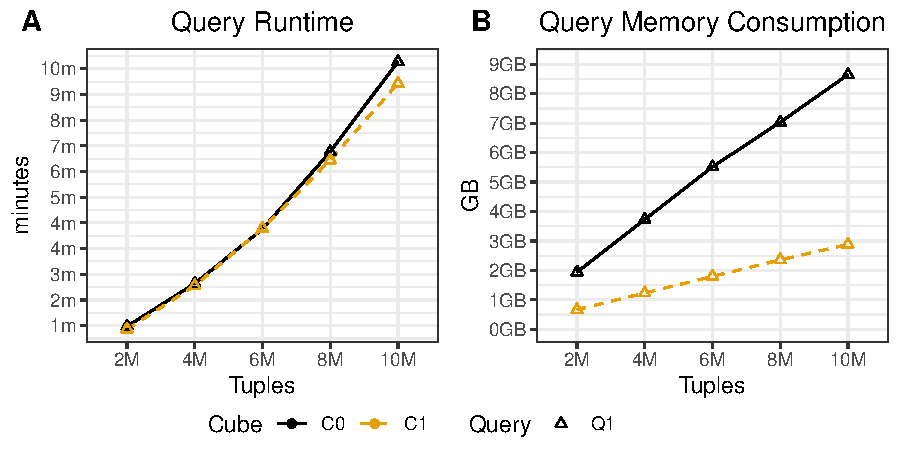
\includegraphics{Figuras/query1-1.pdf}}
  \end{center}
  \vspace{2mm}
  \legenda{(\textbf{A}) Total time to answer a query, including the time to read the data from the disk, build the cube and then answer the query Q1, with cubes C0 and C1. (\textbf{B}) Total memory consumption to answer Q1 with cubes C0 and C1.}
  \FONTE{Author}
\end{figure}

\hypertarget{q2-1}{%
\subsubsection{Q2}\label{q2-1}}

Figure \ref{fig:query2}-A shows the query response times for query Q2, with the execution of the query in the C0 and C2 cubes.
Here the difference when \(\mathcal{T} =\ensuremath{10^{7}}\) is C2 having a runtime 40\% faster than C0.
Figure \ref{fig:query2}-B shows the query memory difference between C0 and C2 for query Q2.
Again the result is C2 taking only a fraction (14\%) of the same query under C0.

\begin{figure}[H]
  \caption{Query 2 results}\label{fig:query2}
  \vspace{6mm}
  \begin{center}
    \resizebox{13cm}{!}{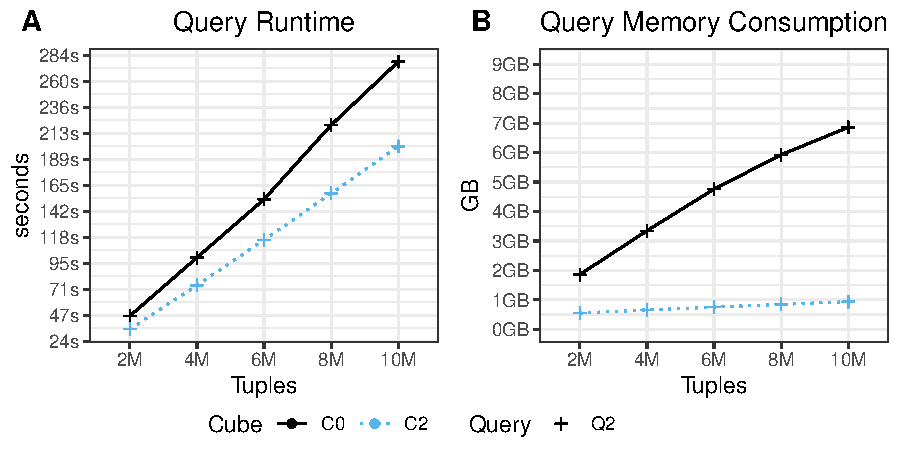
\includegraphics{Figuras/query2-1.pdf}}
  \end{center}
  \vspace{2mm}
  \legenda{(\textbf{A}) Total time to answer a query, including the time to read the data from the disk, build the cube and then answer the query Q2, with cubes C0 and C2. (\textbf{B}) Total memory consumption to answer Q2 with cubes C0 and C2.}
  \FONTE{Author}
\end{figure}

\hypertarget{q3-1}{%
\subsubsection{Q3}\label{q3-1}}

Figure \ref{fig:query3}-A shows the query response times for query Q3, with the execution of the query in the C0 and C3 cubes.
With less inquires and dimensions this operation is expected to be faster, however the speedup is even greater: Q3 under C3 takes only 12\% of the memory used by C0.
Figure \ref{fig:query3}-B shows the query memory difference between C0 and C3 for query Q3, with C3 needing only 7\% of the memory used by C0.

\begin{figure}[H]
  \caption{Query 3 results}\label{fig:query3}
  \vspace{6mm}
  \begin{center}
    \resizebox{13cm}{!}{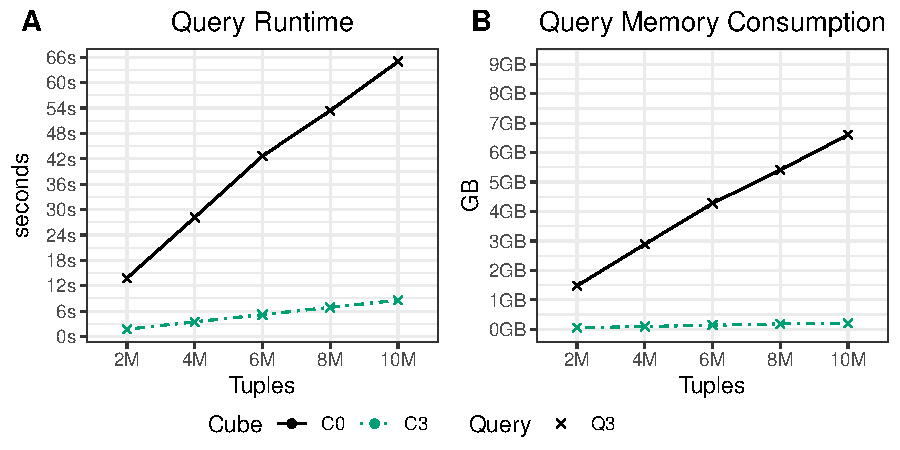
\includegraphics{Figuras/query3-1.pdf}}
  \end{center}
  \vspace{2mm}
  \legenda{(\textbf{A}) Total time to answer a query, including the time to read the data from the disk, build the cube and then answer the query Q3, with cubes C0 and C3. (\textbf{B}) Total memory consumption to answer Q3 with cubes C0 and C3.}
  \FONTE{Author}
\end{figure}

\hypertarget{q4-1}{%
\subsubsection{Q4}\label{q4-1}}

Figure \ref{fig:query4}-A shows the query response times for query Q4, with the execution of the query in the C0 and C4 cubes.
Another query with only two dimensions, and expected to be faster, with C4 taking 5\% of the time used by C0.
Figure \ref{fig:query4}-B shows the query memory difference between C0 and C4 for query Q4, showing the same speedup pattern.

\begin{figure}[H]
  \caption{Query 4 results}\label{fig:query4}
  \vspace{6mm}
  \begin{center}
    \resizebox{13cm}{!}{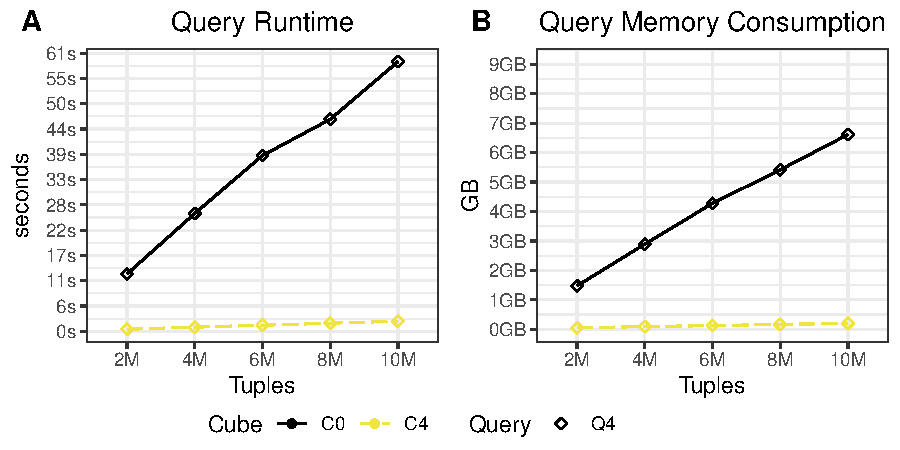
\includegraphics{Figuras/query4-1.pdf}}
  \end{center}
  \vspace{2mm}
  \legenda{(\textbf{A}) Total time to answer a query, including the time to read the data from the disk, build the cube and then answer the query Q4, with cubes C0 and C4. (\textbf{B}) Total memory consumption to answer Q4 with cubes C0 and C4.}
  \FONTE{Author}
\end{figure}

\hypertarget{q5-1}{%
\subsubsection{Q5}\label{q5-1}}

Figure \ref{fig:query5}-A shows the query response times for query Q5, with the execution of the query in the C0 and C5 cubes.
Here with more dimensions than the previous two queries the speedup is less, but still substantial, with C5 taking only 43\% of the runtime used by C0.
Figure \ref{fig:query5}-B shows the query memory difference between C0 and C5 for query Q5, where the same figure of speedups are maintained.

\begin{figure}[H]
  \caption{Query 5 results}\label{fig:query5}
  \vspace{6mm}
  \begin{center}
    \resizebox{13cm}{!}{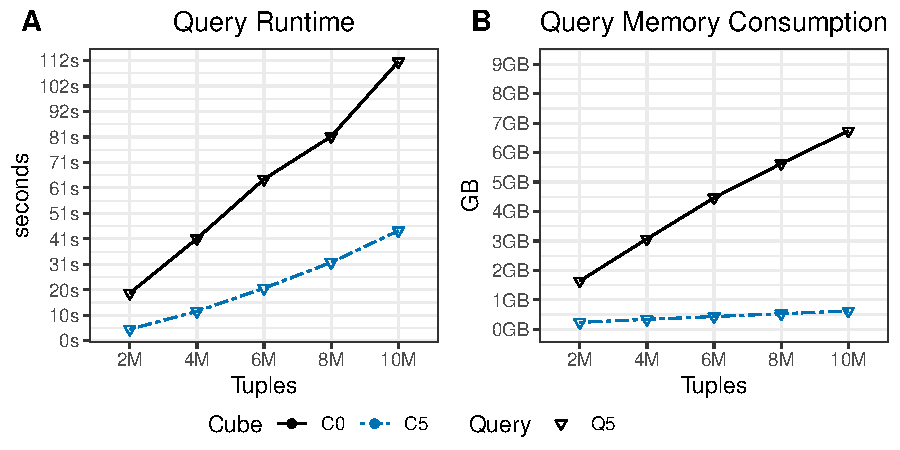
\includegraphics{Figuras/query5-1.pdf}}
  \end{center}
  \vspace{2mm}
  \legenda{(\textbf{A}) Total time to answer a query, including the time to read the data from the disk, build the cube and then answer the query Q5, with cubes C0 and C5. (\textbf{B}) Total memory consumption to answer Q5 with cubes C0 and C5.}
  \FONTE{Author}
\end{figure}

\section{Summary and Analysis}\label{ch:querypart:summary}

For this experiment, the time dimension has the property of having a cardinality that is approximately equal to the amount of tuples (\(\mathcal{C}_d = \mathcal{T}\), for a cardinality of dimension \(d\) and with a database of \(\mathcal{T}\) tuples), as each observation is time-stamped and therefore unique.
This creates a considerable skew to the results with all telemetries, as with \(\ensuremath{10^{7}}\) tuples, a single dimension with \(\mathcal{C}_d = {10}^7\) is not suitable to be computed entirely, and very different from the other dimensions that have a maximum cardinality of \(\mathcal{C}_d = 256\).
As this time dimension was not considered in any query, this is expected to have been one of the reasons for the great difference in memory consumption between the queries and $C0$.

In summary, these results show that building the cube with only the dimensions for a given query can yield up to 80 times less memory for the cube construction, and using between 1\% to 33\% less memory to answer the same query on the same data, with variations depending on the amount of inquired dimensions.
The speedup is so apparent that it'd be \emph{faster} to read, build and then answer a query using one of the low-dimensional cubes (\(C1-5\)) than to directly query an already built data cube with all dimensions (\(C0\)), and is the main contribution of this work.
Furthermore, the shell fragment size parameter shows little benefit in reducing the memory consumption of the queries when they are performed in this manner, and should be kept at 1.

It is also important to highlight the query definitions with the help of a domain expert: most queries are low dimensional in nature, in line with Frag-Cubing's strengths.
These queries are non-exhaustible and meant to be samples, but show that the common algorithmic approaches are suitable for the domain and can be made to improve memory implementation requirements.

